O projeto da Eole Water não fornece todos os dados de especificação da ventoinha que está localizada aproximadamente no centro do topo da torre eólica, nem ao fundo. A única informação possível de ser adotado foi a taxa de fluxo de ar que passa pela ventoinha original, o qual é de 30000 $m^3$/h. 
	Com tal parâmetro a ventoinha foi escolhida:
	Modelos: DQ 1000-8 ou DR 1000-8  da fabricante Rosenberg\cite{axair}
	
	\begin{itemize}
		
		\item Ambas possuem um diâmetro de 1000 mm de ventoinha e 1170 de suporte lateral, com proteção de grade na entrada da ventoinha. Possuem largura de no máximo 330 mm;
		\item O peso varia de 74 a 70 kg;
		\item Voltagem de 280 V a 400 V para se adequar aos 30000 $m^3$/h necessários;
		\item Frequência de 50Hz;
		\item Temperatura de operação $45\,^{\circ}\mathrm{C}$,;
		\item Potência de 2,15 kW;
		\item Velocidade de 8,9 m/s a 10 m/s.		
	\end{itemize}
	
Estrutura:

	\begin{figure}[!htbp]
	 \centering
	  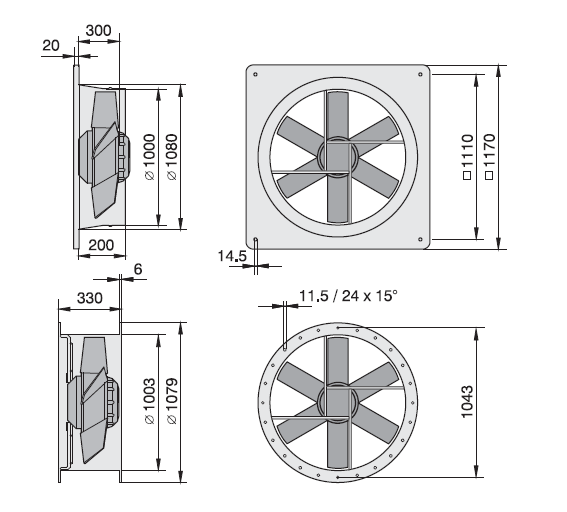
\includegraphics[scale=0.5]{editaveis/figuras/estrutura_ventoinha}
	  \caption[Imagem da estrutura da ventoinha]{Imagem da estrutura da ventoinha\footnotemark}
	  \label{estrutura_ventoinha}
	\end{figure}
	\FloatBarrier
	\footnotetext{Disponível em: http://www.axair-fans.co.uk/assets/product-resources/download/Axair\%20Fans\%20-\%20Rosenberg\%20Selection\%202013.pdf}
	
Grafico de Pressão, Fluxo de ar e Tensão de ambos os modelos:

	\begin{figure}[!htbp]
	 \centering
	  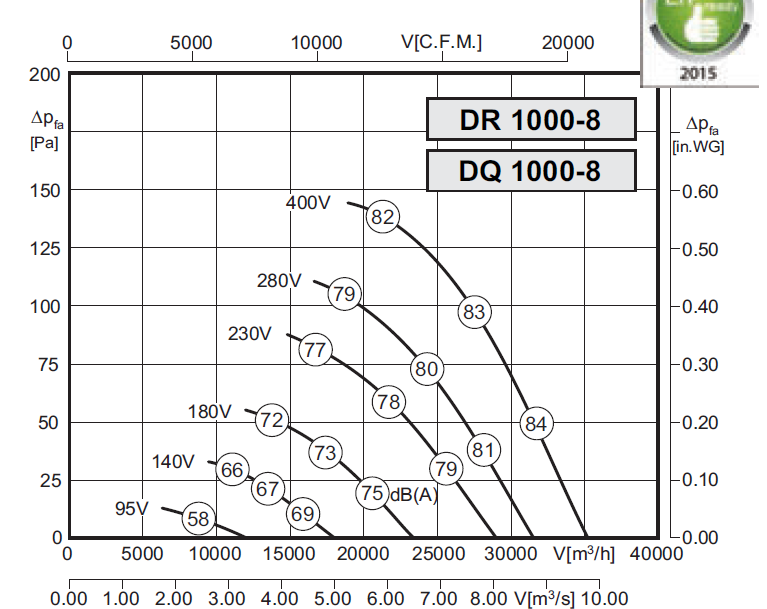
\includegraphics[scale=0.5]{editaveis/figuras/grafico_pressao_fluxo_ar}
	  \caption[grafico de pressão, fluxo de ar e tensão]{grafico de pressão, fluxo de ar e tensão\footnotemark}
	  \label{grafico_pressao_fluxo_ar}
	\end{figure}
	\FloatBarrier
	\footnotetext{Disponível em: http://www.axair-fans.co.uk/assets/product-resources/download/Axair\%20Fans\%20-\%20Rosenberg\%20Selection\%202013.pdf}